% !TeX root = ../INTO-CPS-Manifesto.tex

\section{The INTO-CPS Industrial Case Studies}\label{sec:casestudies}

\fbox{Stylianos Basagiannis}

\subsection{Integrated product-production co-simulation for cyber-physical production system (iPP4CPPS) } 

The case study involved the virtual design and validation of a CPS-based manufacturing system for assembling USB sticks, inspired from Continental's real manufacturing and testing processes in a production line. It is a representative example of distributed heterogeneous systems in which products, manufacturing resources, orders and infrastructure are all cyber-physical. In this setting, several features (such as asynchronous communication, messages flow, autonomy, self-adaptation, etc.) could be investigated at design time, for example using a collaborative modelling approach. Consequently, the case study offered a balance between being sufficiently simple to be easily followed as a production line example, including generating a tangible output, and at the same time being sufficiently general to allow the study of the co-simulation complexity. Furthermore, by choosing a USB stick, the example opened the (unexplored) possibility of extending the purpose of the study to interactions between generated hardware and generated software solutions in the production line.

Obviously, this small experiment, in terms of scale and time, could not give a full and clear assessment of benefits for developing an integrated product-production co-simulation for CPS-based industrial control. Nevertheless, there were some recognisable benefits compared to the current state of technology:

\begin{itemize}
\item the possibility to simulate, test and validate from a holistic perspective and with an increased level of accuracy an entire production system that needs cross-functional expertise; The initial development of a homogeneous co-simulation in VDM for the iPP4CPPS prototype was particularly useful in driving cooperation and making clear the assumptions of the distributed teams involved in modelling the specific components. This phase proved to be the most difficult and time-consuming in building the co-simulation, requiring a very intensive communication for a shared understating of the requirements. Once the VDM co-simulation was running, the independent developments of units could be integrated, validated and deployed in any order.
\item to a certain extent, the ability to handle unpredictable integration requirements. The employment of co-simulations when designing an automated production system avoided the build-up inertia of subsequent design constraints, facilitating the low and late commitment for these decisions, i.e.\ the specific microcontrollers or PLCs, the layout of the plant, the number of memory boxes from the warehouse etc. For example, the possibility to generate code - from all the simulation tools used in this experiment (i.e.\ 4DIAC, 20-Sim, Overture) -- for an extended set of computational devices was a clear advantage in respect to late commitment for the computational system used in the production system. 
\end{itemize}

The methodology adopted in the IPP4CPPS project to develop the co-simulation closely followed the classical stages of agent-oriented or component-based software engineering methodologies. Following the mechanical model derived from the requirements, the high-level abstraction for the behaviour of each simulation was implemented and the interactions among the components could be analysed. It included distinct simulations for each component type (Table 1): production (i.e.\ warehouse station, robot, transporting wagons, and testing station), orders (i.e.\ placed via mobile devices), and factory infrastructure (i.e.\ part tracker). 

The co-simulation model had been initially implemented in VDM and validated on the INTO-CPS tools chain. The main goal of this implementation was manifold: a) to validate the interaction protocols among the composite simulations; b) to have an early working co-simulation where the specific simulations may be gradually added, tested and validated; c) to allow for a more independent development among the dispersed teams involved in modeling the specific simulations, while at the same time keeping the co-simulation functional at all times; and d) to cover the left-over parts of the co-simulation whose modelling was not needed in detail for the validation of the interaction protocol (e.g. test station) or for which there is was FMI-compliant tool (i.e.\ factory infrastructure).   

\begin{table*}[ht]
	\centering
		\begin{tabular}{|p{2.4cm}|p{1.8cm}|p{3.2cm}|p{4cm}|}\hline
			\textbf{Component type} & \textbf{Unit} & \textbf{Technology} & \textbf{Deployment}\\
			\hline\hline
			Orders & HMI & 4DIAC + MQTT \textit{or} Overture (VDM) & smartphones and tablets \\ \hline
			Infrastructure & Part Tracker & Overture (VDM) & NVIDIA Tegra Jetson\\ \hline
			Production & Warehouse + Robotic Arm & 20-sim & Raspberry Pi with UniPi Expansion Board + Stäubli robot\\ \hline
			Production & Wagons & 4DIAC & Raspberry Pi controlling DC motors, position sensors and anti-collision ultrasonic sensors \\ \hline
			Production & Test Station & 4DIAC & Cognex Vision Insight 1100 camera connected to Raspberry Pi for actuators control\\ \hline
			General & Unity & 20-sim animation & PC\\\hline
		\end{tabular}
	\caption{Technologies used for different system components}
	\label{tab:iPP4CPPS_technologies}
\end{table*}

The detailed model of each simulation covered a continuous-time model realised in 20-Sim for the warehouse and robotic arm, a discrete-time model in 4DIAC for the transportation system and test station, and a discrete-time model in Overture for the infrastructure. All units modelled and tested by the heterogeneous co-simulation were then deployed in a demo stand for fine tuning under real-life conditions (Table \ref{tab:iPP4CPPS_technologies}). This phase presumed the extension of code generation capabilities of the simulation tools, such as: 20-sim 4C has been extended with MQTT, Modbus, I2C color sensor, I2C multiplexer and UniPi board for the Raspberry Pi; Overture for employing MQTT as communication protocol on a Raspberry Pi 3; and 4DIAC for accelerometers control. 

\begin{figure}[!ht]
	\centering
		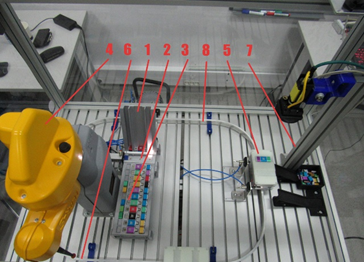
\includegraphics[width=0.9 \textwidth]{./figures/demo_stand}
	\caption{Demo stand for deployment of the co-simulated units, containing: 1) the warehouse stacks; 2) the assembly box at the base of the warehouse stacks; 3) the memory boxes of the warehouse unit; 4) the robotic arm for moving parts around the warehouse; 5) wagons on different locations of the track; 6) the loading station; 7) the test station; 8) the circular track for the wagons..}
	\label{fig:demo_stand}
\end{figure}

The experiment assessed the benefits and the maturity level of model-driven engineering technologies for future adoption into CPS-based production systems. It covered the entire engineering life-cycle (i.e. from requirements to deployment into a real infrastructure) and contributed to several advancements of engineering methods and tools. The experiment delivered an effective proof-of-concept for model-driven engineering of CPS-based production system as a feasible and promising approach to (re)engineer the factory of the future with the employed technologies (i.e.\ INTO-CPS, Overture, 20-Sim and 4DIAC). Nevertheless, the experiment also identified a number of issues that may have further impact over the adoption of model-driven engineering technologies into real settings: the FMI-compatibility of the simulation tools used in industry; the hardware/software-in-the-loop simulations still display complex synchronisation problems for dissimilar time-scales; the extended set of low-level devices (i.e.\ sensors, industrial communication standards etc.) that are used in today and future industry require special standardisation effort to enhance the deployment capabilities of the simulation tools\footnote{More information can be found at \url{http://centers.ulbsibiu.ro/incon/index.php/ipp4cpps/} and \url{http://www.cpse-labs.eu/experiment.php?id=c3_uk_gs_ipp4cpps}.}

